\documentclass{standalone}
\usepackage{tikz}

\usetikzlibrary{positioning}

\begin{document}
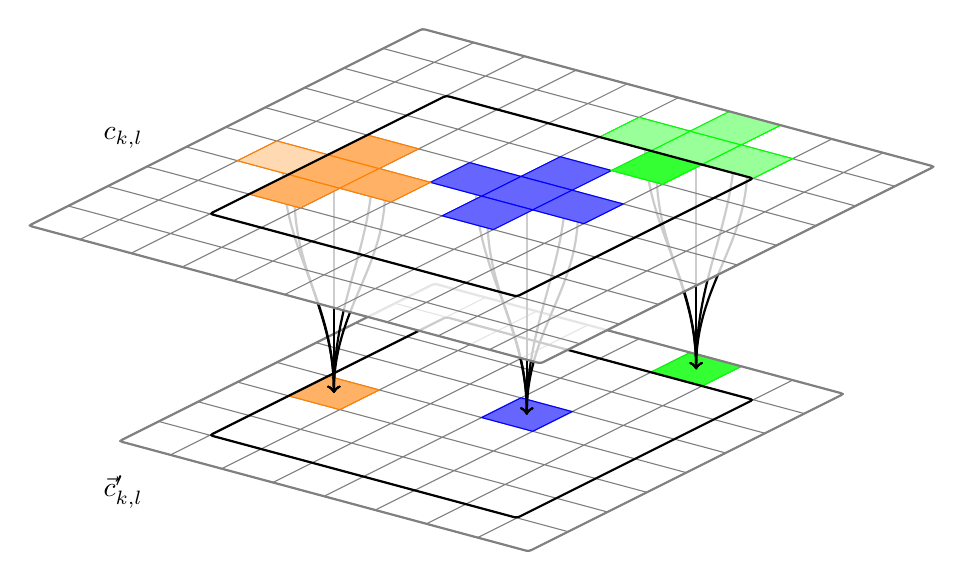
\begin{tikzpicture}[scale=1,every node/.style={minimum size=0.5cm},on grid]

  \begin{scope}[
      yshift=-100,
      every node/.append style={yslant=0.5, xslant=-1.3},
      yslant=0.5,
      xslant=-1.3
    ]
    \coordinate (c42) at (2.25, 1.25);
    \coordinate (c32) at (1.75, 1.25);
    \coordinate (c22) at (1.25, 1.25);
    \coordinate (c33) at (1.75, 1.75);
    \coordinate (c31) at (1.75, 0.75);

    \coordinate (co15) at (0.75, 2.75);
    \coordinate (co25) at (1.25, 2.75);
    \coordinate (co35) at (1.75, 2.75);
    \coordinate (co24) at (1.25, 2.25);
    \coordinate (co26) at (1.25, 3.25);

    \coordinate (co51) at (2.75, 0.75);
    \coordinate (co61) at (3.25, 0.75);
    \coordinate (co71) at (3.75, 0.75);
    \coordinate (co60) at (3.25, 0.25);
    \coordinate (co62) at (3.25, 1.25);
  \end{scope}

  \begin{scope}[
      yshift=-180,
      every node/.append style={yslant=0.5, xslant=-1.3},
      yslant=0.5,
      xslant=-1.3
    ]
    \coordinate (cp32) at (1.75, 1.25);
    \coordinate (cop25) at (1.25, 2.75);
    \coordinate (cop61) at (3.25, 0.75);
  \end{scope}

  % lower plane
  \begin{scope}[
      yshift=-180,
      every node/.append style={yslant=0.5, xslant=-1.3},
      yslant=0.5,
      xslant=-1.3
    ]
    \draw[step=5mm, thin, gray] (-0.5,-0.5) grid (3.5,3.5);

    \fill[blue!60] (1.5,1) rectangle (2.0,1.5);
    \node at (cp32) [draw, color=blue] {};%{$c^\prime_{3,2}$};

    \fill[orange!60] (1.0,2.5) rectangle (1.5,3.0);
    \node at (cop25) [draw, color=orange] {};%{$c^\prime_{2,5}$};

    \fill[green!80] (3.0,0.5) rectangle (3.5,1.0);
    \node at (cop61) [draw, color=green] {};%{$c^\prime_{6,1}$};

    \draw[black,thick, rounded corners=1] (0,0) rectangle (3,3);
    \draw[gray,thick, rounded corners=1] (-0.5,-0.5) rectangle (3.5,3.5);
  \end{scope}

  % arrows
  \begin{scope}
    \draw[>->, thick] (c31) node[left,scale=1.3] {} to[out=270,in=90] (cp32);
    \draw[>->, thick] (c32) node[left,scale=1.3] {} to[out=270,in=90] (cp32);
    \draw[>->, thick] (c33) node[left,scale=1.3] {} to[out=270,in=90] (cp32);
    \draw[>->, thick] (c22) node[left,scale=1.3] {} to[out=270,in=90] (cp32);
    \draw[>->, thick] (c42) node[left,scale=1.3] {} to[out=270,in=90] (cp32);

    \draw[>->, thick] (co24) node[left,scale=1.3] {} to[out=270,in=90] (cop25);
    \draw[>->, thick] (co25) node[left,scale=1.3] {} to[out=270,in=90] (cop25);
    \draw[>->, thick] (co26) node[left,scale=1.3] {} to[out=270,in=90] (cop25);
    \draw[>->, thick] (co15) node[left,scale=1.3] {} to[out=270,in=90] (cop25);
    \draw[>->, thick] (co35) node[left,scale=1.3] {} to[out=270,in=90] (cop25);

    \draw[>->, thick] (co51) node[left,scale=1.3] {} to[out=270,in=90] (cop61);
    \draw[>->, thick] (co61) node[left,scale=1.3] {} to[out=270,in=90] (cop61);
    \draw[>->, thick] (co71) node[left,scale=1.3] {} to[out=270,in=90] (cop61);
    \draw[>->, thick] (co62) node[left,scale=1.3] {} to[out=270,in=90] (cop61);
    \draw[>->, thick] (co60) node[left,scale=1.3] {} to[out=270,in=90] (cop61);
  \end{scope}

  % upper plane
  \begin{scope}[
      yshift=-100,
      every node/.append style={yslant=0.5, xslant=-1.3},
      yslant=0.5,
      xslant=-1.3
    ]
    \fill[white,fill opacity=0.8] (-1.0,-1.0) rectangle (4.0,4.0);
    \draw[step=5mm, thin, gray] (-1.0,-1.0) grid (4.0,4.0);

    \fill[blue!60] (2,1) rectangle (2.5,1.5);
    \node at (c42) [draw, color=blue] {};%{$c_{4,2}$};

    \fill[blue!60] (1.5,1) rectangle (2.0,1.5);
    \node at (c32) [draw, color=blue] {};%{$c_{3,2}$};

    \fill[blue!60] (1,1) rectangle (1.5,1.5);
    \node at (c22) [draw, color=blue] {};%{$c_{2,2}$};

    \fill[blue!60] (1.5,1.5) rectangle (2.0,2.0);
    \node at (c33) [draw, color=blue] {};%{$c_{3,3}$};

    \fill[blue!60] (1.5,0.5) rectangle (2.0,1.0);
    \node at (c31) [draw, color=blue] {};%{$c_{3,1}$};

    \fill[orange!60] (0.5,2.5) rectangle (1.0,3.0);
    \node at (co15) [draw, color=orange] {};%{$c_{1,5}$};

    \fill[orange!60] (1.0,2.5) rectangle (1.5,3.0);
    \node at (co25) [draw, color=orange] {};%{$c_{2,5}$};

    \fill[orange!60] (1.5,2.5) rectangle (2.0,3.0);
    \node at (co35) [draw, color=orange] {};%{$c_{3,5}$};

    \fill[orange!60] (1.0,2.0) rectangle (1.5,2.5);
    \node at (co24) [draw, color=orange] {};%{$c_{2,4}$};

    \fill[orange!30] (1.0,3.0) rectangle (1.5,3.5);
    \node at (co26) [draw, color=orange] {};%{$c_{2,6}$};

    \fill[green!80] (2.5,0.5) rectangle (3.0,1.0);
    \node at (co51) [draw, color=green] {};%{$c_{5,1}$};

    \fill[green!40] (3.0,0.5) rectangle (3.5,1.0);
    \node at (co61) [draw, color=green] {};%{$c_{6,1}$};

    \fill[green!40] (3.5,0.5) rectangle (4.0,1.0);
    \node at (co71) [draw, color=green] {};%{$c_{7,1}$};

    \fill[green!40] (3.0,0.0) rectangle (3.5,0.5);
    \node at (co60) [draw, color=green] {};%{$c_{6,0}$};

    \fill[green!40] (3.0,1.0) rectangle (3.5,1.5);
    \node at (co62) [draw, color=green] {};%{$c_{6,2}$};

    \draw[black,thick, rounded corners=1] (0,0) rectangle (3,3);
    \draw[gray,thick, rounded corners=1] (-1.0,-1.0) rectangle (4.0,4.0);
  \end{scope}

  \node at (-5cm,-1.5cm) [black] {$c_{k,l}$};
  \node at (-5cm,-6cm) [black] {$\vec{c}^\prime_{k,l}$};
\end{tikzpicture}
\end{document}
